
\documentclass[11pt, a4paper]{article}
\usepackage{graphicx}
\usepackage{amsmath}
\usepackage{listings}


\title{Assignment 3 : Fitting Data to Models} 

\author{Suhas C EE20B132} 

\date{\today} 

\setlength{\parindent}{2em}
\begin{document}		
		
\maketitle 
\section*{Abstract}

In this assignment we aim to :
\begin{itemize}
    \item Reading data from files and parsing them
    \item Analysing the data to extract information
    \item Study the effect of noise on the fitting process
\end{itemize}

\section{Generating the data}

 The data required is generated by running the script \texttt{"generate\_code.py"} script file. This generated a file \texttt{"fitting.dat"}. This file consists of 10 columns each having 100 data points, in which the first column corresponded to time stamp and the remaining columns are data of the noisy functions $f(t) = 1.05J_2(t)-0.105t+n_{\sigma}(t)$, where the noise signal $n_{\sigma}(t)$ is \textit{normally distributed} and its probability distribution is given by:
\begin{equation}
     P(n(t)|\sigma)=\frac{1}{\sqrt{2\pi\sigma^2}}e^{-\frac{n(t)^2}{2\sigma^2}} \label{eq:1}
\end{equation}

\section{Analyse the data}

We know the actual function to be fitted which is given by,

\begin{equation}\label{eq:2}
  f(t)=1.05J_2(t)-.105t
  \end{equation}
where $J_2(t)$ is the \textit{Bessel Function of the first kind of Order 2}. We can plot it’s graph also using the \texttt{pyplot} library by knowing the data points over a specific period of time. We define a python function $g(t, A, B)$ defined as follows:
  
\begin{verbatim}
    def g(t, A, B):
        return A*sp.jn(2,t) + B*t
\end{verbatim}

We keep the time period same for all the plots and it is defined by:

\texttt{t = linspace(0,10,101)}
\newline

On plotting the true function’s value along with all the 9 noise added values, the following plot was generated:

  \begin{figure}[!tbh]
   	\centering
   	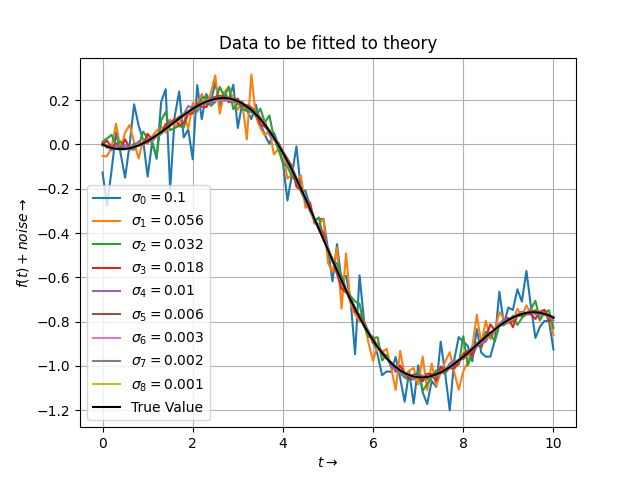
\includegraphics[scale=0.5]{figure0.png}  
   	\caption{Noisy Data with True Data}
   	\label{fig:fig1}
   \end{figure} 

As we can see from Figure~\ref{fig:fig1}, the “noisiness” of the data increases with increasing value of $\sigma$. 

Another view of how the noise affects the data can be seen below: 

  \begin{figure}[!tbh]
   	\centering
   	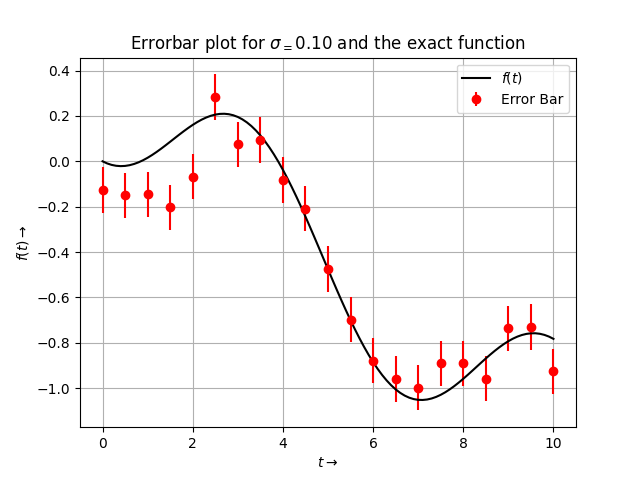
\includegraphics[scale=0.5]{figure1.png}  
   	\caption{Noisy Data with Errorbar}
   	\label{fig:fig2}
   \end{figure} 
   
The blue lines (error bar) indicate the deviation of the noisy data from the original data, at that value of t. It is plotted at every 5th point to make the plot readable else the plot would have been clumsy.

\section{The Matrix equation}
The function which we need to approximate can also be computed by means of a matrix equation. We obtain the function $g(t,A,B)$ as a column vector using the following matrix equation:
\begin{equation}\label{eq:3}
    g(t,A,B) = M.p
\end{equation}
where the matrix
\begin{equation}
M=\left[\begin{matrix}
J_2(t_1)&t_1\\
...&...\\
J_2(t_m)&t_m
\end{matrix}\right]\text{, }
p=\left[\begin{matrix}
A\\B
\end{matrix}\right]
\end{equation}

While performing the computation of the function we generate the matrix M and compute $M.p$ and get the function output.

\section{Best fit approximation to the noisy data}

From the data given to us we see that, we must approximate the noisy data to a function of the form:

\begin{equation}\label{eq:4}
    g(t, A, B) = AJ_2(t)+Bt
\end{equation}

where we must find the values of the constants A and B by using the least square estimation. For this purpose we take the value of A = 0,0.1,0.2,...,2 and B = -0.2,-0.19,...,0 and iterate through each of the above values of A and B, and finally get the mean squared error between the given noisy data and the approximated function by taking the each pair of above values of A and B. 
\newline

The error is computed by means of the following equation:
\begin{equation}\label{eq:5}
    \epsilon_{ij} = \frac{1}{101}\sum_{k=0}^{101}(f(t_k) - g(t_k, A_i, B_j))^2
\end{equation}

where $\epsilon_{ij}$ is the error for $(A_i,B_j)$.

After computing the mean squared error we plot a contour plot for the same with the values of A and B on the x-axis and y-axis respectively. The plot is as shown below:

\begin{figure}[!tbh]
   	\centering
   	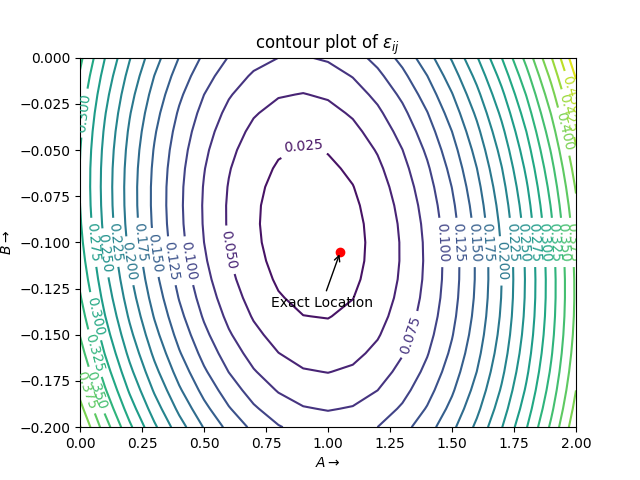
\includegraphics[scale=0.5]{figure2.png}  
   	\caption{Contour Plot of $\epsilon_{ij}$}
   	\label{fig:fig3}
   \end{figure} 
   
   
\section{Performing the Least error fit}

We are required to find the best measure estimate for the constants A and B in the equation \eqref{eq:3} for the noisy data. We do this by applying the method of least square estimation. This is implemented in python by using the \texttt{lstsq()} function from the \texttt{scipy} package. We pass the matrix M and the noisy data as the input to the \texttt{lstsq()} function and we get the best fit values of A and B. We perform this for all the 9 random noise added data.
\newline

We then compute the mean squared error in the coefficients A and B to their actual value of \texttt{A0 = 1.05} and \texttt{B0 = -0.105} and plot the same  against the standard deviation of the random noise. The plot is shown below:

\begin{figure}[!tbh]
   	\centering
   	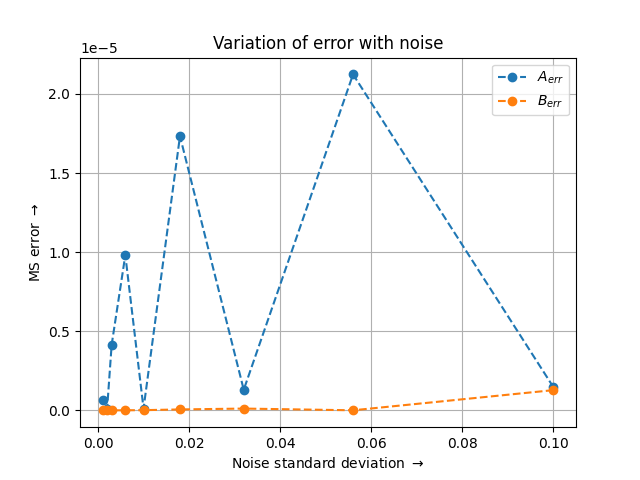
\includegraphics[scale=0.5]{figure3.png} 
   	\caption{Mean squared error vs Noise Standard deviation}
   	\label{fig:fig4}
   \end{figure} 

We aren't able to seek in much information to get a relation between $\sigma and$ $\epsilon$ from the above plot. If we plot the same in \texttt{log-log} scale along with their error bar, the plot looks like:

\begin{figure}[!tbh]
   	\centering
   	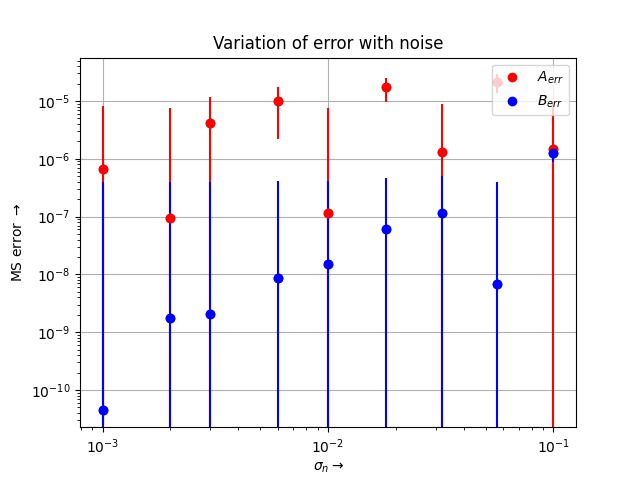
\includegraphics[scale=0.5]{figure4.png} 
   	\caption{Mean squared error vs Noise Standard deviation log-log plot}
   	\label{fig:fig5}
   \end{figure} 
 
 From the above plot we can infer that there is a linear relation between $\sigma_n$ and $\epsilon$, which is the required result to be produced.

\section{Conclusion}
We have used the given noisy data and computed the best possible for the underlying model parameters by minimizing the mean squared error. By plotting the mean squared error between the estimated model parameters A and B and the true value function's parameters A0 and B0, we see that this error is varying linearly with the standard deviation of the noise added to true value.
\end{document}
